
\documentclass[a4paper,11pt]{article}
\usepackage{a4wide}
\usepackage[utf8x]{inputenc}
\usepackage{ucs}
\usepackage[T1]{fontenc}
\linespread{1.2}
\usepackage{courier}

\usepackage{subcaption}
\usepackage{graphicx} % Allows figures
\usepackage{amsmath}%,amssymb,amsthm,amsfonts,ulem}
\usepackage{hyperref}
\usepackage{float}
\usepackage{mdwlist}
\usepackage{wrapfig}
\usepackage{caption}
\usepackage{todonotes}

\usepackage{tikz}
\usepackage{pgf-umlsd}

%Section style
\usepackage{etoolbox} %for configuration of sloppy
\usepackage{xcolor, colortbl}

% usage: \graphicc{width}{file}{caption}{label}
\newcommand{\graphicc}[4]{\begin{figure}[H] \centering
            \includegraphics[width={#1\textwidth}, keepaspectratio=true]{{#2}}
            \caption{{#3}} \label{#4} \end{figure}}

\newcommand{\mc}[2]{\multicolumn{#1}{c}{#2}}
\definecolor{Gray}{gray}{0.85}
\definecolor{secnum}{RGB}{102,102,102}

\makeatletter
    \def\@seccntformat#1{\llap{\color{secnum}\csname the#1\endcsname\hskip 16pt}}
\makeatother
%end section style

{\sloppy}{\hbadness 10000\relax}{}{} %adds hbadness to sloppy

 
% Frontpage stuff
\title{Deliverable 5 - Project Course: Development Studio 2014 \\ Team India 
\includegraphics[width=.04\textwidth]{img/india.png}}
\author
{
    Martin Jørgensen \\ 
    University of Copenhagen \\
    Department of Computer Science \\
    {\tt tzk173@alumni.ku.dk}
    \and
    Henrik Bendt \\
    University of Copenhagen \\
    Department of Computer Science \\
    {\tt gwk553@alumni.ku.dk}
    \and
    Kasper Passov \\
    University of Copenhagen \\
    Department of Computer Science \\
    {\tt pvx884@alumni.ku.dk}
    \and
    Lasse Ahlbech Madsen \\
    University of Copenhagen \\
    Department of Computer Science \\
    {\tt xsc606@alumni.ku.dk}
}
\date{\today}

\begin{document}

\maketitle

\tableofcontents
\pagebreak
\section{Project Data}
\begin{table}[h!]
    \begin{tabular}{l|l|l}
        \textbf{Item}     & \textbf{URL}                              & \textbf{Revision}\\\hline
        Code Experimental & \url{https://github.com/martinnj/PCDS}    & \texttt{TODO}\\
        Code Production   & \url{https://github.com/martinnj/Leapkit} & \texttt{TODO}\\
        Scrum board       & \url{https://trello.com/b/lF49jIHe}       & \texttt{See Figure \ref{fig:backlog}}
    \end{tabular}
    \label{tab:projdata}
    \caption{For access to the board/repositories, please contact any group member.}
\end{table}

\section{Sprint Report}
% stories completed, progress report (e.g., through a burndown chart), next sprint

\subsection{Current Sprint}

The following stories was completed as planed at the start of the sprint:
\begin{itemize}
    \item Create code that can save the translated LinkedIn data to the Leapkit Database.
    \item Setup Jenkins environment
    \item Implement basic match making algorithm ready for iterative developement/extensions
    \item Create test suite for the code generated in the previous sprint.
\end{itemize}

\begin{figure}[!ht]
    \centering
    \begin{subfigure}[b]{0.5\textwidth}
        \scalebox{.6}{\begin{tikzpicture}

% horizontal axis
    \draw[->] (0,0) -- (8,0) node[anchor=north] {\emph{Day}};
% labels
    \draw   (0,0) node[anchor=north] {0}
            (1,0) node[anchor=north] {1}
            (2,0) node[anchor=north] {2}
            (3,0) node[anchor=north] {3}
            (4,0) node[anchor=north] {4}
            (5,0) node[anchor=north] {5}
            (6,0) node[anchor=north] {6}
            (7,0) node[anchor=north] {7};

% vertical axis
    \draw[->] (0,0) -- (0,8) node[anchor=east] {\emph{Points remaining}};
% labels
    \draw   (0,1) node[anchor=east] {3}
            (0,2) node[anchor=east] {5.5}
            (0,3) node[anchor=east] {8}
            (0,4) node[anchor=east] {10.5}
            (0,5) node[anchor=east] {12}
            (0,6) node[anchor=east] {15.5}
            (0,7) node[anchor=east] {18};

% projected 
    \draw[thick, dotted, red] (0,7) -- (7,0);

% actual
    \draw[thick, blue] (0,7) -- (1,6.5) -- (2,6.0) -- (3,4) -- (4,2.5) -- (5,2.5) -- (6,1); 
   
% legend
    \begin{scope}[shift={(4,4)}] 
        \draw[thick, dotted, red] (0,0) -- (0.5,0) 
            node[black, right]{Projected Sprint};
        \draw[thick, blue, yshift=\baselineskip] (0,0) -- 
            plot[] (0.25,0) -- (0.5,0)
            node[black, right]{Actual Sprint};
    \end{scope}
\end{tikzpicture}
}
        \caption{Burndown of the current sprint}
        \label{fig:burndownSprint}
    \end{subfigure}%
    \begin{subfigure}[b]{0.5\textwidth}
        \scalebox{.7}{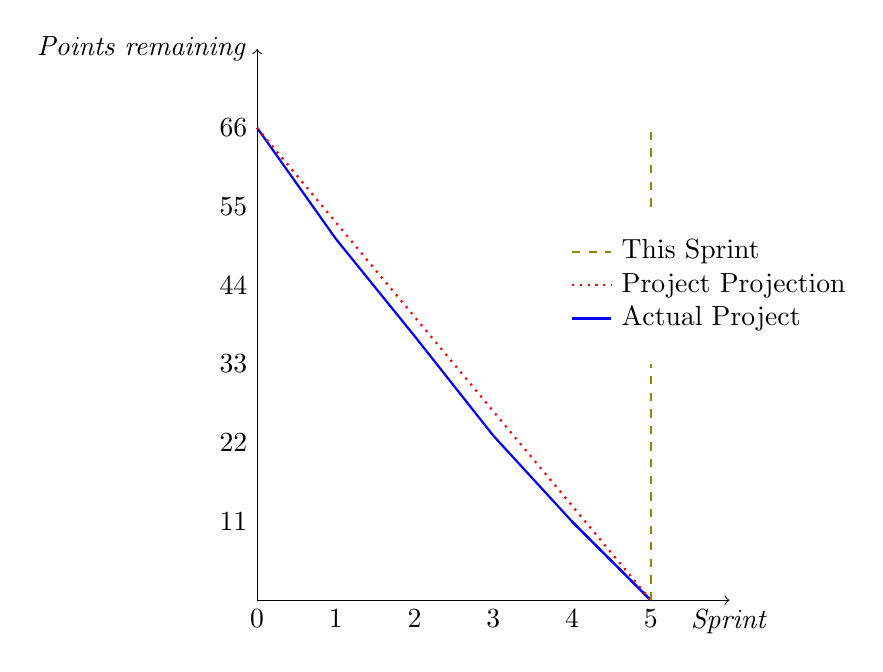
\begin{tikzpicture}

% horizontal axis
    \draw[->] (0,0) -- (6,0) node[anchor=north] {\emph{Sprint}};
% labels
    \draw   (0,0) node[anchor=north] {0}
            (1,0) node[anchor=north] {1}
            (2,0) node[anchor=north] {2}
            (3,0) node[anchor=north] {3}
            (4,0) node[anchor=north] {4}
            (5,0) node[anchor=north] {5};

% vertical axis
    \draw[->] (0,0) -- (0,7) node[anchor=east] {\emph{Points remaining}};
% labels
    \draw   (0,1) node[anchor=east] {11}
            (0,2) node[anchor=east] {22}
            (0,3) node[anchor=east] {33}
            (0,4) node[anchor=east] {44}
            (0,5) node[anchor=east] {55}
            (0,6) node[anchor=east] {66};
% actual
    \draw[thick, blue] (0,6) -- (1,4.59) -- (2,3.355) -- (3,2.09)-- (4,1.00) -- (5,0);
% actual projected
    \draw[thick, dashed, blue] (4,1.00) -- (5,0);

% projected 
    \draw[thick, dotted, red] (0,6) -- (5,0);


% current sprint 
    \draw[thick, dashed, olive] (5,0) -- (5,3);
    \draw[thick, dashed, olive] (5,5) -- (5,6);


    
\begin{scope}[shift={(4,4)}] 
    \draw[thick, dotted, red] (0,0) -- (0.5,0) 
        node[black, right]{Project Projection};
    \draw[thick, blue, yshift=\baselineskip * - 1] (0,0) -- (0.5,0)
        node[black, right]{Actual Project};
    \draw[thick, dashed, olive, yshift=\baselineskip] (0,0) -- (0.5,0)
        node[black, right]{This Sprint};
\end{scope}

\end{tikzpicture}
}
        \caption{Burndown of the project}
        \label{fig:burndownProject}
    \end{subfigure}
    \caption{Burndown charts}
\end{figure}

\subsection{Next Sprint}
Next sprint will focus on integration of the current into the Leapkit solution. After this integration, the matchmaking algorithm can iteratively be expanded and CI will be the focus point. The remaining backlog items can be siin in Figure \ref{fig:backlog}
\begin{itemize}
\item Finish database design and implementation
\item Integrate LinkedIn redirection and extraction
\item Integrate database solution
\item Integrate match making solution
\item Further expansion on match making algorithm
\end{itemize}

\graphicc{0.4}{img/backlog.png}{The current project backlog.}{fig:backlog}
\section{Sprint Retrospective}
% what went well, what went less well, and what will you improve

We established a good connection to our project partners and had a
couple of meetings where we met everyone in the company. We have firmly
established what the project is about and the scope of the project.

We managed to complete almost all of our original sprint goals (and added some later), but the work load was a bit lighter than intended. So we did a descent estimation of the time score of the backlog items handled in this sprint.

Jenkins got set up after we started programming and is not fully ready for use, but by the start of the next sprint, we expect to have it up and running. This was due to underestimating the time to setup the virtual machine with the Leapkit environment, which should be included in the CI environmet. We do however have Jenkins setup to handle our (at the moment) seperate python code, but we still need to develop a rigid test suite.

The Scrum Master did not assign tasks to individual people in the
group. Instead people assigned themselves to the tasks they felt like
doing. In the future we will seek to make this assignment in the
initial sprint meeting and adjust these at the workdaily Scrum meetings,
such that the the workload is better balanced between the group members.

People have been bad at meeting at the agreed time, so we will try to improve this. The fairly noticeable difference in peoples' arrival time have caused our work schedules to become rather ad hoc and our workdaily Scrum meetings to be later on the day instead of the initial task (for those who arrive on time). This will definitely need to be changed in the upcoming sprint.

\section{Sprint Goal}

%TODO Report on the sprint goal by describing your current development process and by discussing how and why you have improved/will improve the proces.

The developement process is roughly as follows. A set of tasks are created from a set of sprint goals, whereby the sprint goals are split into smaller, more concrete tasks, typically solvable by one or two developers. The tasks are then given a time frame using Scrum techniques such as planning poker, and afterwards assigned to the developers. This is done by the Scrum master via dialog and in agreement in the team. 

A task is then solved a developer (or a team of developer if needed), and the results are loosely presented to the rest of the team, so everybody is up to date on the current progress. The task is then moved to either the Done list or the Need Testing/Review list, for further testing or reviewing, before either improving/changing the solution based on the review or move it to Done, if the tests where successful.

Thus far, the test and review part of the development process has been very light and of little focus. This can be improved by e.g. forcing other developers, i.e. not the ones who produced the solution, to test/review the solution. Not only will this force the team to focus on quality ensurance and making intelligent solutions, it might also affect the quality of the tests. A tester, who has no knowledge of how the solution works, is not affected by the ideas and assumptions behind this solution and might create testing scenarios covering cases the producing developer had not thought of.


\end{document}
